\documentclass[a4paper,12]{exam}
\usepackage[right=0.75cm, left=0.75cm, top=0.75cm, bottom=1.5cm]{geometry}
\usepackage[utf8]{inputenc} % para acentos
\usepackage{amsmath, amsfonts, amssymb} %para forrmas matemáticas
\usepackage{graphicx} %pacote para o uso de figuras
\usepackage[portuguese]{babel} %para os rótulos automáticos fiquem em português
\usepackage{adjustbox}
\usepackage{multirow}
\usepackage{multicol}
\usepackage{fourier} %transforma a fonte utilizada no latex
\usepackage{tikz}
\usepackage{tabularx}
\usepackage{chemfig}
\usepackage{isotope}%para escrever os isótopos
\usepackage[version=4]{mhchem} %bioquímica
\usepackage{chemformula} %fórmula químicas
\usepackage{elements} %para a distribuição eletrônica.
\usepackage{xymtexpdf}%PDF Mode para moléculas complexas
\usepackage{epic,carom} %pacote do colesterol
\usepackage{xymtex} %desenha fórmulas químicas estruturais
\usepackage{enumitem} %para trocar os rótulos dos itens
\usepackage{siunitx} %para usar unidades do sistema intenacional
\usepackage{mathrsfs} %letras para notações matemática


\author{Fred Klier}
\newcommand{\class}{Química}
\newcommand{\term}{2021}
\newcommand{\examnum}{Exercícios de Química}
\newcommand{\examdate}{\today}
\newcommand{\timelimit}{90 minutos}
\newcommand{\examauthor}{Fred Klier}

\pgfdeclarelayer{background}
\pgfdeclarelayer{main}

\pgfsetlayers{background,main}

\pagestyle{headandfoot}
\firstpageheader{}{}{}
\runningheader{}{}{}
\firstpagefooter{\class}{\examnum\ - Page \thepage\ of \numpages}{\term}
\firstpagefootrule
\runningfooter{\class}{\examnum\ - Page \thepage\ of \numpages}{\term}
\runningfootrule

\begin{document}

\begin{tikzpicture}[remember picture, overlay] %remember picture permite chamar nodes que não estão no mesmo ambiente tikzpicture e overlay permite passar as margens definidas.

	\node(logo) at (current page.north east) [anchor=north east,xshift=-0.25cm, yshift=-0.5cm] {
\includegraphics[width=6cm]{cnsm.png}};
	
	\node(nomealuno) at (logo.north west) [anchor=north east]{{\textbf{Nome:}}{\makebox[11cm]{\hrulefill}\textbf{N$^{\circ}$:}}{\makebox[1cm]{\hrulefill}}};
	
	%\node(nota) at (logo.north west) [anchor=north east,xshift=-0.01cm, yshift=-0.5cm]{\textbf{Nota:}{\makebox[1cm]{\hrulefill}}};
	
	\node(dataprova) at (logo.north west) [anchor=north east,xshift=-0.1cm, yshift=-1cm]{Data de aplicação:{\makebox[.1cm]{}}{\makebox[0.6cm]{\hrulefill}}/{\makebox[0.6cm]{\hrulefill}}/\term};
	
	\node(datadev) at (logo.north west) [anchor=north east,xshift=-0.01cm, yshift=-1.6cm]{Data da devolução:{\makebox[.1cm]{}}{{\makebox[0.6cm]{\hrulefill}}/{\makebox[0.6cm]{\hrulefill}}/\term}};
	
	%\node(valor) at (nota.north west) [anchor=north east,xshift=0cm, yshift=0cm] {\textbf{Valor: 30} {\makebox[1.7cm]{}}};
	
	\node(turma) at (logo.north west) [anchor=north east,xshift=-9.94cm, yshift=-.5cm]{2$^{\circ}$ Ano do Ensino médio};
	
	\node(prova) at (turma.south west) [anchor=north west,xshift=0cm, yshift=-.1cm]{\examnum};
	
	\node(professor) at (datadev.north west) [anchor=north east,xshift=-4.8cm, yshift=0cm]{Professor(a): \examauthor};


\end{tikzpicture}

\vspace{1.2cm}
\rule{18cm}{1pt}
%\fbox{$[substância] =\mathscr{M}=\frac{n_1}{V_{(l)}} =\frac{m_1}{M_1  \ast  V_{(l)}}$} \\




\begin{multicols}{2}
  	\begin{questions}
	  \question A farinha de linhaça dourada é um produto natural que
	  oferece grandes benefícios para o nosso organismo. A maior
	  parte dos nutrientes da linhaça encontra-se no óleo desta
	  semente, rico em substâncias lipossolúveis com massas
	  moleculares elevadas. A farinha também apresenta altos
teores de fibras proteicas insolúveis em água, celulose,
	  vitaminas lipossolúveis e sais minerais hidrossolúveis.
	  Considere o esquema, que resume um processo de
	  separação dos componentes principais da farinha de 
	  linhaça dourada. 
	  
	  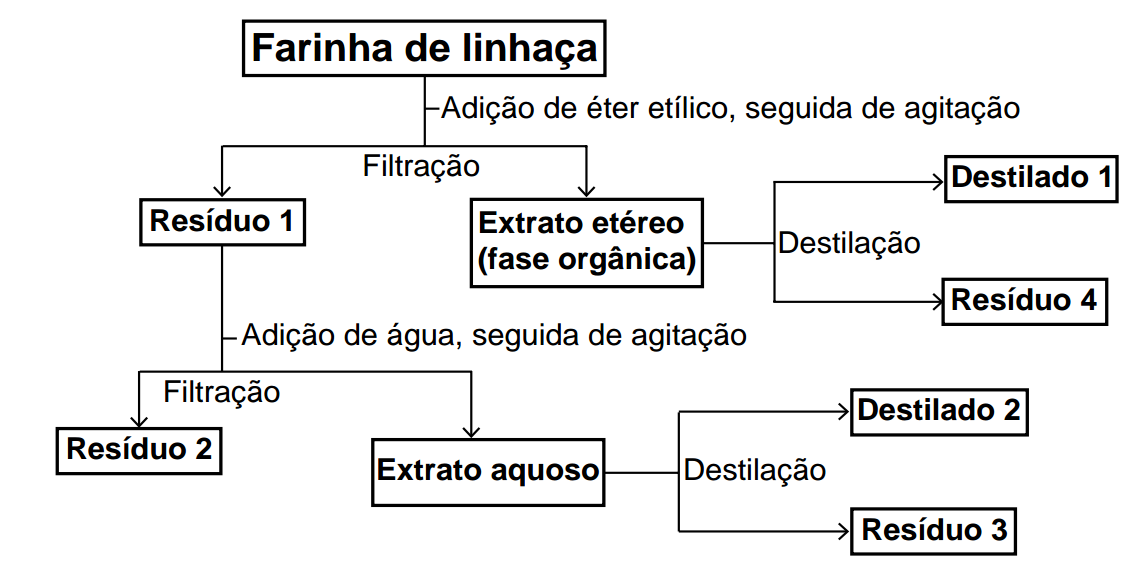
\includegraphics[width=8cm]{farinha.png}
		
		\begin{enumerate}[label=\alph*)]
	  	\item Explique o que é esperado no "destilado 2".
	  	\fillwithlines{8em}
	   	\item Enumere os fenômenos físicos nesse processo? 
	   	\fillwithlines{8em}
	   	\item Explique se os fenômenos físicos são endotérmicos ou exotérmicos?
	   	\fillwithlines{8em}
		\end{enumerate}
	
	
	  \question O petróleo é uma fonte de energia de baixo custo
	  e de larga utilização como matéria-prima para uma 
	  grande variedade de produtos. É um óleo formado
	  de várias substâncias de origem orgânica, em sua
	  maioria hidrocarbonetos de diferentes massas molares.
	  São utilizadas técnicas de separação para a obtenção
	  dos componentes comercializáveis do petróleo.
	  Além disso, para aumentar a quantidade de frações
	  comercializáveis, otimizando o produto de origem fóssil,
	  utiliza-se o processo de craqueamento. nesse processo moléculas grandes são quebradas em moléculas menores. 
	  
	  \begin{enumerate}[label=\alph*)]
	  \item Explique o processo utilizado para a separação do petróleo.
	  \fillwithlines{8em}
	  \item Explique como o craqueamento vai afetar o resultado da separação.
	  \fillwithlines{8em}
	  \end{enumerate}	
		
	 \end{questions}
\end{multicols}
\end{document}
